\chapter{合乘情形下的最少车辆数}
\label{chap:share}
一方面,随着科学技术的发展,无人驾驶车辆正在逐渐走进人们的生活。自上世纪七十年代开始,英国、美国等国家就在无人驾驶车辆的研究生那个取得了较为瞩目的成果,而我国在2005年,第一辆城市无人驾驶汽车在上海交通大学研制成功。近些年来,随着信息技术的飞速发展,计算机视觉等领域突破性成果的出现,无人驾驶技术的研发也取得了卓越的成果。在不久的将来,我们将迎来无人驾驶车辆的市场化,彼时,路面上的无人驾驶车辆将不断地增加,有人驾驶车辆将被逐渐地取代。人们将会越来越愿意购买并使用无人驾驶车辆。
\par
无人驾驶车辆相对于有人驾驶车辆来说,可以有更多的操控性,不同的车辆之间可以更好的通过网络连接等手段传递信息,车辆的交通行为将会发生改变。无人驾驶车辆上的车载感应器,可以和智能交通系统联合工作,优化道路交叉口的车流量,交通信号灯可以更好的调度控制,改善车辆的出行效率,环节交通拥堵。同时,无人驾驶车辆的出现可以减少由于人的失误造成的交通事故。因此,对于交通领域的研究者来说,无人驾驶车辆的出现,将会带来很多可以研究的新兴问题,许多传统的问题在无人驾驶车辆的情形下也会有新的挑战。
\par
另一方面,近些年来,Airbnb和Uber等公司通过共享经济的思维把人类社会的经济模式推广到了互联网社会,通过互联网和移动设备连接了不同用户的经济行为,并且取得了很大的成功。Airbnb使得原来私人的房屋成为共享住宿服务的场所,Uber利用平台的预约功能实现车座位的共享,不同的乘客可以拼车共享。ofo,摩拜单车等公司将单车共享,使得原本私人化的单车成为临时所有物,与别人共享。这样的共享模式,使得人们可以以更低的成本得到相同的服务,同时节约了资源,减少了路面上行驶的车辆,从而进一步减少了交通拥堵,更进一步减少了尾气排放,大气污染。这样的经济模式值得推广,也给交通领域的研究者带来了许多问题可以进行研究。
\par
研究数据显示,在Uber等平台的拼车服务中,实际上每辆车的平均载客数为1.3左右,依然接近于一人一车的模式,这违反了平台提供这样的服务的初衷。因此,如何设计较为有效的算法匹配乘客和调度车辆,设计较好的平台运行机制就成为了一个重要的研究问题。本章节即是想探讨,在可以合乘的情形下,未来城市中需要多少的车辆才能服务到所有的乘客。

\section{数据来源}
我们从廊坊市,天台市,银川市,等城市采集了出租车,公交车等车辆的出行数据,包括,出行的出发地点,出发时间,到达地点,到达时间等。在数据预处理中,我们剔除了出租车和公交车等的数据,留下了私人车的出行数据,并且将出发地点和到达地点的地理位置信息都对应到了最近的交叉路口,每个城市的美俄个交叉路口都有编号,在预处理后的数据中,以编号代替交叉路口的地理位置。出发时间和到达时间都转换成秒。具体的数据解释见下表~\ref{tab:triplist}。
\begin{table}
    \centering
    \caption{出行数据的具体解释}
    \label{tab:triplist}
  \begin{tabular}{|c|p{10cm}|}
    \hline
    数据项 & 具体解释\\
    \hline \hline 
    tripRowid & 出行数据的索引,但是不是按照时间顺序排列的\\
    \hline 
    oTime & 出行的出发时间,将时间转化为秒,一天中最小的为0秒,最大的为86400秒\\
    \hline 
    dTime & 出行的到达时间,将时间转化为秒,一天中最小的为0秒,最大的为86400秒\\
    \hline 
    oInter & 出行的出发地点,将地点转化为交叉口编号,在之后的计算中出行的地理位置信息,都按照交叉口的地理信息计算\\
    \hline 
    dInter & 出行的到达地点,将地点转化为交叉口编号,在之后的计算中出行的地理位置信息,都按照交叉口的地理信息计算\\
    \hline 
  \end{tabular}
\end{table}

\par
为了计算不同出行地点之间的行驶时间,我们在将地理信息转换成最近的交叉路口信息的同时,通过百度地图API获得了不同交叉路口之间的行驶时间,生成了一个出行时间矩阵,用于之后的建模计算中。该数据表中的数据信息如表~\ref{tab:odtime}~所示。

\begin{table}
  \centering
  \caption{交叉路口之间的出行时间}
  \label{tab:odtime}
  \begin{tabular}{|c|c|}
  \hline 
  数据项 & 具体解释\\
  \hline \hline 
  o & 出发交叉口的编号\\
  \hline 
  d & 到达交叉口的编号\\
  \hline 
  time & 根据百度地图API得到的从o到d的汽车行驶时间\\
  \hline 
  \end{tabular}
\end{table}

\section{合乘判别条件}
\subsection{算法设计}
在我们的数据中,部分城市的数据,对于每个出行有其相对应的乘客数量数据,但是由于实际上,每辆车的乘客数量的平均值为1.3人,我们可以合理的假设每个出行的乘客数量都为1.因为在这里我们为了简化问题以便于讨论,我们只考虑两个出行合乘的情形,现在路面上的大部分车都为四座以上的车型,因此,假设每个出行只有一个乘客是合理的,可以满足我们讨论问题的需要。
\par
对于两个出行,如果想要通过合乘将两个出行合并为一个出行,这两个出行之间必须满足一定的时间和空间关系。
\par
时间上,首先出发的出行的到达时间必须在第二个出发的出行的出发时间之后,否则,若首先出发的出行的到达时间较早,则这两个乘客不会出现在同一辆车上,因为第一个乘客在第二个乘客出发前就可以到达自己的目的地。在数据中,我们将实际的到达时间视作为,在合乘的框架下,乘客的预计到达时间。我们希望在考虑合乘时,减少了交通拥堵,乘客的出行效率提高,所以,我们希望合乘下,每个乘客都可以在自己的预计到达时间内到达目的地。但是如果到达的太早,可能也会给乘客造成困扰。比如,如果乘客是想去电影院看电影,但是由于出行效率增加,比自己的预计到达时间提前到了半个小时。对于乘客来说,没有这半个小时或许会更好。所以,我们希望在提前到的前提下,不能提前到达太多。
\par
空间上,由于选择合乘,原本针对一个乘客规划的行车路线,需要同时再考虑另外一个乘客的出行。对于已经在车上的乘客而言,为了去接另一位乘客,可能需要偏离自己本来的行车路线,绕路到别的地方。在考虑合乘的系统框架下,乘客是接受绕路的,因为在合乘系统里,绕路是默认设定,乘客可以因为绕路而获得折扣,从而抵回损失。但是,即使这样,乘客不能接受绕路太多,因为乘客损失的时间成本不能被经济的补偿而抵回。所以,我们不允许绕路太多。对于后上车的乘客而言,如果第一位乘客的预计到达时间比第二位乘客的预计到达时间早,车辆就需要先去送第一位乘客,从而第二位乘客的路线就会绕路,同样的,我们也不允许第二位乘客绕路太多。
\par
下面,我们将严格化的说明上述想法。为此,我们分为两种情况分别讨论。
\par
在进行讨论之前,我们先引入一些记号,以使得讨论更加严格和准确。使用到的符号都列在表~\ref{tab:notation}~中。
\begin{table}
\centering
\caption{记号及其含义说明}
\label{tab:notation}
\begin{tabular}{|c|c|}
\hline 
符号 & 含义\\
\hline 
\hline
$Tr$ & 所有出行的集合 \\
\hline 
$I_i^o$ & $Tr$中的第$i$个出行$tr_i$的出发交叉路口的编号\\
\hline 
$I_i^d$ & $Tr$中的第$i$个出行$tr_i$的到达交叉路口的编号\\
\hline 
$t_i^o$ & $Tr$中的第$i$个出行$tr_i$的出发时间\\
\hline 
$t_i^d$ & $Tr$中的第$i$个出行$tr_i$的到达时间\\
\hline 
$\delta$ & 允许提前到达的时间阈值\\
\hline
$\Delta$ & 允许绕路的距离因子\\
\hline 
$\epsilon$ & 路径重合率因子\\
\hline 
\texttt{travel} & 计算行驶时间的函数\\
\hline 
\end{tabular}
\end{table}
\par
以下,以$tr_1$记为第一个出行,$tr_2$记为第二个出行。
\begin{itemize}
\item 当一个乘客的出行路线包含了另一个乘客的出行路线时,即如图~\ref{fig:cover1}~所示的情形,由于第一个出行需要在$t_1^d$之前到达,并且不可以提前太早,所以有
\begin{equation}
  t_1^d - \delta < t_1^o + travel(I_1^o,I_2^o,I_2^d,I_1^d) < t_1^d
\end{equation}
同样地,由于第二个出行也需要在$t_2^d$之前到达,并且不能提前太早,所以有
\begin{equation}
  t_2^d - \delta < t_1^o + travel(I_1^o,I_2^o,I_2^d) < t_2^d
\end{equation}
\par
对于第一个乘客而言,和二号乘客合乘之后需要绕路,但是也不能绕路太远,所以有
\begin{equation}
travel(I_1^o,I_2^o,I_2^d,I_1^d) < \Delta \times travel(I_1^o,I_1^d)
\end{equation}

      \begin{figure}
      \centering
      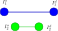
\includegraphics[width=6cm]{./figures/img/coverage1.pdf}
      \caption{第一个乘客的路线覆盖了第二个乘客的路线}
      \label{fig:cover1}
      \end{figure}

\item 当一个乘客的出行路线与另一个乘客的出行路线相交但互不包含时,即如图~\ref{fig:cover2}所示,由于第一个出行需要在$t_1^d$之前到达,并且不可以提前太早,所以有
\begin{equation}
  t_1^d - \delta < t_1^o + travel(I_1^o,I_2^o,I_1^d) < t_1^d
\end{equation}
同样地,由于第二个出行也需要在$t_2^d$之前到达,并且不能提前太早,所以有
\begin{equation}
  t_2^d - \delta < t_1^o + travel(I_1^o,I_2^o,I_1^d,I_2^d) < t_2^d
\end{equation}
\par
对于第一个乘客而言,和二号乘客合乘之后需要绕路,但是也不能绕路太远,所以有
\begin{equation}
travel(I_1^o,I_2^o,I_1^d) < \Delta \times travel(I_1^o,I_1^d)
\end{equation}
同样地,二号乘客和一号乘客合乘后,也不能绕路太远,所以有
\begin{equation}
travel(I_2^o,I_1^d,I_2^d) < \Delta \times travel(I_2^o,I_2^d)
\end{equation}
\par
同时,当在两个出行的路线重合率较低时,即在距离第一位乘客的终点较近的时候需要绕路去接第二位乘客,对于第一位乘客而言较为不公平,所以在我们的判断条件中,我们不允许,所以路径的重合率有最低的要求。
\begin{equation}
travel(I_1^o,I_2^o) < \epsilon \times travel(I_1^o, I_1^d)
\end{equation}

      \begin{figure}
      \centering
      \includegraphics[width=10cm]{./figures/img/coverage2.pdf}
      \caption{第一个乘客的路线与第二个乘客的路线相交,但互不包含}
      \label{fig:cover2}
      \end{figure}
\end{itemize}

\par
将以上想法写成算法伪代码如算法~\ref{alg:isshare}~所示。
\begin{algorithm}[htbp]
\SetAlgoLined
\SetKwInOut{Input}{Input}\SetKwInOut{Output}{Output}
\caption{isShareable($tr_i,tr_j$)}
\label{alg:isshare}
\BlankLine
$tr_1,tr_2\leftarrow $为两个出行\;
\uIf{$I_i^o > I_j^o$}{
  $tr_1 \leftarrow tr_j$\;
  $tr_2 \leftarrow tr_i$\;
}
\uElse{
  $tr_1 \leftarrow tr_i$\;
  $tr_2 \leftarrow tr_j$\;
}
\uIf{$t_1^d > t_2^d$}{
  \uIf{$t_1^o + travel(I_1^o,I_2^o) < t_2^o$}{
    \uIf{($t_1^d - \delta < t_1^o + travel(I_1^o,I_2^o,I_2^d,I_1^d)$) and ($t_1^o + travel(I_1^o,I_2^o,I_2^d,I_1^d) < t_1^d$)}{
      \uIf{($t_2^d - \delta < t_1^o + travel(I_1^o,I_2^o,I_2^d)$) and ($t_1^o + travel(I_1^o,I_2^o,I_2^d) < t_2^d$)}{
        \uIf{$travel(I_1^o,I_2^o,I_2^d,I_1^d) < \Delta\times travel(I_1^o,I_1^d)$}{
          return True\;
        }
        \uElse{
          return False\;
        }
      }
    }
  }
}
\uElse{
  \uIf{($t_1^d < t_2^d$) and ($t_1^d > t_2^o$)}{
    \uIf{$t_1^o + travel(I_1^o,I_2^o) < t_2^o$}{
      \uIf{($t_1^d - \delta < t_1^o + travel(I_1^o,I_2^o,I_1^d)$) and ($t_1^o + travel(I_1^o,I_2^o,I_1^d) < t_1^d$)}{
        \uIf{($t_2^d - \delta < t_1^o + travel(I_1^o,I_2^o,I_1^d,I_2^d)$) and ($t_1^o + travel(I_1^o,I_2^o,I_1^d,I_2^d) < t_2^d$)}{
          \uIf{$travel(I_1^o,I_2^o,I_1^d) < \Delta\times travel(I_1^o,I_1^d)$}{
            \uIf{$travel(I_2^o,I_1^d,I_2^d) < \Delta\times travel(I_2^o,I_2^d)$}{
               \uIf{$travel(I_1^o,I_2^o) < \epsilon \times travel(I_1^o,I_1^d)$}{
                return True\;
              }
              \uElse{
                return False\;
              }
            }
          }
        }
      }
    }
  }
}
return False\;
\end{algorithm}

\subsection{算法时间复杂度分析}
从算法~\ref{alg:isshare}~可以知道,算法中只有\texttt{if-else}的条件判断语句和赋值语句,除了调用了\texttt{travel}函数之外,都只是加法和大小比较。并且,由于我们将交叉路口之间的行驶时间处理成了一个矩阵,并且进一步将其处理成了Hash表$Dis$,使得查询其中的一个元素的时间复杂度变为$O(1)$,所以算法总共的时间复杂度为$O(1)$。


\section{网络生成算法}
\subsection{算法设计}
上一部分,我们介绍了如何设计合理的判断两个出行是否可以合乘的条件,在时间上和空间上都加了限制,最终提出了算法~\ref{alg:isshare}~进行判断。在这一部分,我们将利用算法~\ref{alg:isshare}~进行网络的生成。
\par
每一个出行都可以视为网络上的一个节点,我们只需要对每两个节点进行判断,就可以决定它们之间是否有边相连,所以就有与算法~\ref{alg:genegraph}~类似的算法~\ref{alg:genegraphshare}。
\begin{algorithm}[htbp]
\SetAlgoLined
\SetKwInOut{Input}{Input}\SetKwInOut{Output}{Output}
\caption{generateGraph($Tr$)}
\label{alg:genegraphshare}
\BlankLine
初始化有向图网络$G \leftarrow \emptyset$\;
\For{$tr_i$ in $Tr$}{
  \tcp{$Tr(k:)$代表索引在$k$及以后的出行的集合;}
  \For{$tr_j$ in $Tr(i+1:)$}{
    \uIf{isShareable($tr_i, tr_j$)}{
      $G\leftarrow G\cup \{(tr_i, tr_j)\}$\;
    }
  }
}
return $G$\;
\end{algorithm}

\subsection{算法时间复杂度分析}
容易知道,若令$m = |Tr|$,则上述算法一共进行了$\frac{m(m-1)}{2}$次循环,每次循环中的语句,包括函数\texttt{isShareable}都是$O(1)$的,所以算法的总共的时间复杂度为$O(\frac{m(m-1)}{2})$。由于想要得到完整的网络,我们必须对$Tr$中的所有出行组成的所有出行对进行判断是否有边,由于有$m$个出行数据,我们就必须进行至少$\frac{m(m-1)}{2}$次比较。故此算法的时间复杂度只能为$O(\frac{m(m-1)}{2})$。

\section{求解所需最少车辆数}
从前两部分可以知道,生成的图以及最终生成的图都与第~\ref{cha:num}~章中类似,所以我们可以通过类似的方式,引入定义,定理和证明,说明在生成的图上寻找需要的最少车辆数和在图上寻找最大匹配时等价的。
\subsection{原问题等价于在图上寻找最大匹配}
我们希望用尽可能少的车辆服务到所有的出行,并且假定每个合乘有且仅有两个出行,所以当选择合乘的人数越多的时候,所需要的车辆就越少。这是因为,和原来的车辆数相比,一旦一名乘客合乘成功,路面上就可以减少一辆车。当减少的车辆最多时,剩下的车辆就最少。所以,直观上,在原网络中寻找最少的车辆等价于寻找最大的匹配。我们可以根据以下的定理证明。
\begin{theorem}
在原问题中求解所需最少的车辆数,等价于,在根据算法~\ref{alg:genegraphshare}~生成的图中寻找最大匹配。
\end{theorem}
\begin{proof}
设$G = (N, E)$为根据算法~\ref{alg:genegraphshare}~生成的图,$M$为$G$上的一个匹配。则想要服务到所有的乘客所需要的最少车辆数$c$为
\begin{equation}
c = |N|-2|M|+|M| = |N|-|M|
\end{equation}
所以,
\[
  \min c \Longleftrightarrow \max |M|
\]
\end{proof}

\subsection{带花树算法求解原始图上的最大匹配}
带花树算法是一个在一般图上寻找最大匹配的算法,其主要想法是在图中寻找一个有匹配边和未匹配边组成的奇圈,即花,将花进行压缩成一个点,构成新的图,在新的图上寻找增广路,以增加匹配的数量,最终得到图上的最大匹配。带花树算法的时间复杂度为$O(|N|^3)$。

\subsection{生成收缩图}
在用带花树算法进行了最大匹配的求解之后,我们可以根据求解得到的最大匹配,将匹配的出行对进行合并。因为这两个乘客选择合乘,他们都在同一辆车上,我们可以将这个组合出行看成是从最早出行的乘客的出发地点出发到最晚到达的乘客的到达地点的一次出行。所以我们可以将这两个出行所代表的图上的节点以及它们之间的边合并为一个节点。原始图根据最大匹配进行收缩后得到的收缩图的结构发生了很大的改变,我们将以两个算法分别说明如何根据匹配的结果对出行进行合并,以及如何生成收缩图。

\begin{algorithm}[htbp]
\SetAlgoLined
\SetKwInOut{Input}{Input}\SetKwInOut{Output}{Output}
\caption{combineNodes($G,\mathcal{M}$)}
\label{alg:combnode}
\BlankLine
$Tr^\prime \leftarrow \emptyset$\;
\For{$(u,v) \in \mathcal{M}$}{
  $tr_u\leftarrow $为$u$所代表的出行\;
  $tr_v\leftarrow $为$v$所代表的出行\;
  $tr_n\leftarrow $为一个新的出行\;
  $t_n^o \leftarrow \min(t_u^o,t_v^o)$\;
  $t_n^d \leftarrow \max(t_u^d,t_v^d)$\;
  $I_n^o \leftarrow I_{\argmin(t_u^o,t_v^o)}^o$\;
  $I_n^d \leftarrow I_{\argmax(t_u^o,t_v^o)}^d$\;
  $Tr^\prime \leftarrow Tr^\prime \cup \{tr_n\}$\;
}

\For{$v \in N$ and $v \notin \mathcal{M}$}{
  $Tr^\prime \leftarrow Tr^\prime \cup v$\;
}
return $Tr^\prime$\;
\end{algorithm}

\par
以上,我们根据最大匹配结果得到了合并出行后的所有出行。根据这些出行,我们再次利用\texttt{isShareable}进行判断两个出行是否可以合乘,就得到了新的图。算法如算法~\ref{alg:contract}。

\begin{algorithm}[htbp]
\SetAlgoLined
\SetKwInOut{Input}{Input}\SetKwInOut{Output}{Output}
\caption{contractedGraph($Tr^\prime$)}
\label{alg:contract}
\BlankLine
初始化无向图网络$G^\prime \leftarrow \emptyset$\;
对$Tr^\prime$中的出行按照出发时间进行排序\;
\For{$tr_i$ in $Tr^\prime$}{
  \tcp{$Tr^\prime(k:)$代表索引在$k$及以后的出行的集合;}
  \For{$tr_j$ in $Tr^\prime(i+1:)$}{
    \uIf{isShareable($tr_i, tr_j$)}{
      $G^\prime\leftarrow G^\prime\cup \{(tr_i, tr_j)\}$\;
    }
  }
}
return $G^\prime$\;
\end{algorithm}



\subsection{将无向图转换成二分图}
对于一般的无向图,我们不能将其转换成二分图,但是由于出行数据具有一定的特殊性,每条数据都包含了出行的出发地点和到达地点,我们可以将出发地点和到达地点分别视为图中的一个节点。并且,只在不同出行的到达节点和出发节点之间加无向边。由此得到的图即是二分图。算法~\ref{alg:convertshare}~展示了以上的想法。

\begin{algorithm}[htbp]
\SetAlgoLined
\SetKwInOut{Input}{Input}\SetKwInOut{Output}{Output}
\caption{convertToBipartite($G = (N,E)$)}
\label{alg:convertshare}
\BlankLine
$G_b \leftarrow \emptyset$\;
$N_b \leftarrow \emptyset$\;
$E_b \leftarrow \emptyset$\;
\For{$v$ in $N$}{
  $tr_i\leftarrow$$v$所代表的出行\;
  $v_o^i\leftarrow$$tr_i$的出发交叉路口对应的节点\;
  $v_d^i\leftarrow$$tr_i$的到达交叉路口对应的节点\;
  $N_b\leftarrow N_b \cup \{v_i^o,v_i^d\}$\;
}
\For{$e = (u,v)$ in $E$}{
  $tr_i\leftarrow u$所代表的出行\;
  $tr_j\leftarrow v$所代表的出行\;
  $E_b\leftarrow E_b\cup \{(v_i^d, v_j^o)\}$\;
}
return $G_b = (N_b, E_b)$\;
\end{algorithm}


\subsection{Hopcroft-Karp算法求解最小车辆规模}
在前面的部分,我们说明了生成出行图,并且利用带花树算法求解图上的最大匹配。图上的一个匹配即代表了一次合乘出行。我们可以将这两次出行视为一次出行,出行的出发地点即是两次出行中较早出发的乘客的出发地点,到达地点即是最后到达的乘客的到达地点。在进行了图的收缩之后,我们生成了一个基于原始图的收缩图,再利用算法~\ref{alg:convertshare}~将图转换成二分图,之后再二分图上进行求解最小车辆规模。
\par
在收缩图上求解最小车辆规模,就是求解最少的路径覆盖,使得每个出行都被服务到。图上的每个路径都代表了一辆车的先后服务,它分别服务路径上的每一个出行。求解最少的路径覆盖所有的点,就是求解最少的车辆服务所有的出行。即,二者是等价的。这由以下的两个定理保证。
\begin{theorem}\label{theo:pathshare}
对于网络$G = (N, E)$上的一个路径覆盖$\mathcal{C} = \{P_1,\cdots, P_h\}$,所有的出行都可以被服务到。
\end{theorem}

\begin{proof}
对于网络$G = (N,E)$上的一个路径$P= \{e_1 = (n_1^1, n_1^2),\cdots, e_k = (n_k^1,n_k^2)\}$,根据我们生成网络上边的算法,可以知道$n_1^1,n_1^2$(记为$tr_1,tr-2$),两个出行可以被同一辆车服务,并且,按照我们的判别条件,服务$tr_1$的车一定能在$t_2^o$之前到达$I_2^o$接到乘客。因此,出行$tr_2$的出发时间和达到时间没有延误。故和$n_1^2$有边的$n_2^2$所代表的出行不会延误,即车可以在指定时间之前到达出发地接到$n_2^2$代表的出行的乘客。以此类推,路径$P$中的所有$N(P)$个乘客都可以被同一辆车准时服务到,没有出行的延迟。因此,对于路径覆盖$\mathcal{C}$,所有的出行都可以被不同的车服务到。
\end{proof}
\par
以上我们证明了,网络$G = (N, E)$上的一个路径覆盖,如果我们以一辆车代表一个路径,则$G$上的一个路径覆盖即是可以服务所有出行的一个可行解。接下来,我们证明任意一个原问题的可行解,即一个车辆的分配使得所有出行都被服务到,都对应了$G$上的一个路径覆盖。
\begin{theorem}\label{theo:originshare}
对于所有出行的一个车辆分配,在网络$G = (N, E)$中,都存在一个路径覆盖$\mathcal{C} = \{P_1,\cdots, P_h\}$。
\end{theorem}
\begin{proof}
记$T$为所有被分配的车辆的集合,$p_t = \{tr_1,\cdots, tr_{k_t}\}, \forall t \in T$为每辆车所被分配的出行的集合,并且不失一般性的,我们假定车辆$t$即按照$tr_1,\cdots,tr_{k_t}$的顺序接送出行。则由于$tr_1,tr_2$之间满足函数\texttt{isShareable}的判别条件,所以如果将$tr_1,tr_2$都对应为网络中的一个节点,则它们之间有一条边,以此类推。所以如果将$p_t$中的所有出行都对应于网络上的节点,则$P_t = \{e_1 = (n_1^1, n_1^2),\cdots, e_{k_t} = (n_{k_t}^1, n_{k_t}^2)\}$为$G$中的一条路径,并且$P_t$中的每一个节点都代表了一个被服务的出行,其中$n_1^1$代表$tr_1$,$n_i^2, n_{i+1}^1$代表$tr_{i+1}, i = 1,\cdots, k_t$。将所有$P_t$这样的路径组合成一个路径覆盖$\mathcal{C} = \{P_1,\cdots, P_t\}$,则所有出行都在网络的节点中,所有的出行都被服务到。
\end{proof}

\par
以上我们证明了求解最小车辆规模和求解最小路径覆盖的等价性。同时,我们可以证明在收缩图上求解最小路径覆盖等价于在收缩图对应的二分图上求解最大匹配。

\begin{theorem}
在$G_b = (N_b,E_b)$上的最大匹配$M$等价于在$G = (N,E)$上的最小路径覆盖。
\end{theorem}
\begin{proof}
假设$\mathcal{C} = \{P_1,\cdots, P_h\}$为$G$的最小路径覆盖,$\mathcal{M} = \{(u_1,v_1),\cdots, (u_s, v_s)\}$为$G_b$的最大匹配。
\par
由于$\mathcal{C}$为最小路径覆盖,故$h$为所有路径覆盖中最小的值。$\mathcal{C}$中共有$|N| - h$条边,为所有路径覆盖中的最大值。我们将$\mathcal{C}$中的边按照算法~\ref{alg:convertshare}~的方法对应到$G_b$中的边,则$\mathcal{C}$中的每一条边都对应了$G_b$中两个节点的匹配,即$\mathcal{C}$对应了$G_b$中的一个匹配,故$|\mathcal{M}| \geq |N| - h$。
\par
另一方面,对于$\mathcal{M}$中的一个匹配,两个节点分别属于不同出行,并且这两个出行满足\texttt{isShareable}的条件,在$G$中有一条边。将$\mathcal{M}$中的匹配都对应到$G$中,则得到$G$中的一个边的集合$E^\prime$。
\par
在$E^\prime$中,没有两条边有共同的端点。否则,我们可以分两种情况讨论。
\par
两条边若有共同的到达端点,则在$G_b$中,它们对应了相同的在$N_o$中的节点,这与$\mathcal{M}$是一个匹配矛盾。
\par
两条边若有共同的出发端点,则在$G_b$中,它们对应了相同的在$N_d$中的节点,这与$\mathcal{M}$是一个匹配矛盾。
\par
所以$E^\prime$为$G$的一个路径覆盖,从而$ |\mathcal{M}|\leq N-h$。
\par
综上所述,$|\mathcal{M}| = N - h$,即求解$G$中的最小路径覆盖可以转换成求解$G_b$中的最大匹配。
\end{proof}

\par
同时,根据我们生成网络时的算法,以及出行数据的特殊性,我们可以证明生成的网络是有向无环图。
\begin{theorem}
根据全部出行数据$Tr^\prime$,以及判断两个出行是否可以被同一辆车服务的函数\texttt{isShareable},生成的图$G^\prime = (N^\prime,E^\prime)$为DAG。
\end{theorem}
\begin{proof}
假设$P$为图$G^\prime$中的一个有向圈,并且我们可以不妨假设$P$的长度为2,因为长度为0和1的有向圈不存在,可以类似的证明长度大于2的有向圈不存在。
\par
设$P = \{(N_1, N_2), (N_2, N_1)\}$,则
\[
  t_1^d \leq t_2^o < t_2^d \leq t_1^o
\]
\par
但是,根据出行时间的意义,可以知道$t_1^d > t_1^o$,矛盾。
\par
这样我们就证明了$G^\prime$中不存在长度为2的有向圈,同样的可以证明,长度大于2的有向圈也不存在。
\end{proof}

\par
以上我们证明了我们的网络是有向无环图,并且在对应的二分图上求解最大匹配和在图上求解最小路径覆盖是等价的。因此,我们可以利用Hopcroft-Karp算法求解。


\subsection{时间复杂度分析}
在以上的分析中,我们一共使用到了带花树算法,生成收缩图的算法,将收缩图转换成二分图的算法,以及求解最大匹配的Hopcroft-Karp算法。
\par
带花树算法的时间复杂度为$O(|N|^3)$。生成收缩图的算法共两层循环,循环的内部的时间复杂度为$O(1)$,所以算法的总时间复杂度为$O(\frac{|E|(|E|-1)}{2})$。将收缩图转换成二分图的算法含有两个循环,循环的内部的时间复杂度都为$O(1)$,一个循环的循环次数为$|N|$次,另一个循环的循环次数为$|E|$次,所以总时间复杂度为$O(|E|+|N|)$,Hopcroft-Karp算法的时间复杂度为$O(|E|\sqrt{|N|}+|N|)$。
\par
综上,本部分的所有算法的总时间复杂度为$O(|E|\sqrt{|N|}+|N|)$。